\chapter{Particle properties of waves}\label{c2}
A particle is a material body whose dimensions are insignificant in comparison
with the typical dimensions of its motion. A pebble can be considered to be a
particle when one considers its projectile motion but not so when one considers
its rotation. At a more extreme level, the earth is treated like a particle when
one studies it as a part of solar system but not when we study ocean currents.
A wave, on the other hand, is a periodic disturbance. In the case of material
waves the disturbance is felt in properties of the materials. For example, the
passage of a sound waves leads to periodic compressions and rarefactions in the
material. They are detected as changes in the pressure in the case of fluids and
internal stresses in the case of solids. Electromagnetic waves do not need 
materials for their propagation and their passage is manifested in the periodic
variations in electric and magnetic field intensities at a point. Although this
distinction between particles and waves seems quite natural it is not so when 
one observes nature beyond the human senses. Newton considered light to be
particulate and it took more than two centuries to suspect that it is probably
a wave. The interference experiments of Young could be explained only by 
treating light as a wave. Maxwell predicted the existence of electromagnetic
waves and Hertz confirmed their existence. Maxwell also derived the speed of
electromagnetic waves and it was the same as the speed of light. As a result,
light was suspected to be an electromagnetic wave and was indeed shown to be so.
However, at the turn of the century other experiments were conducted whose 
outcome could not be explained by assuming that light is a wave. We shall 
consider a few of them in this chapter.

\section{Black body radiation}\label{c2s1}
Material bodies absorb and emit electromagnetic radiation. When they are in
thermal equilibrium the net absorbtion of radiation matches the net emission.
Most bodies do not absorb all radiation. They reflect or transmit it. Further,
their absorption depends on the angle of incidence. A black body is the one 
that absorbs all radiation irrespective of its wavelength and angle of 
incidence. If a blackbody is at thermal equilibrium then it should emit the
energy it absorbs. The emitted energy is called \emph{black body radiation}.
An approximately black body is a large cavity enclosed in an opaque material 
and with a small hole for radiation to get in. It is only an approximation 
because waves with wavelength greater than the hole's diameter will be 
partially reflected. Further, a finite size cavity cannot hold radiation of all
wavelengths.

Since a black body absorbs radiation of all wavelengths it also emits radiation
of all wavelengths. If $U_\lambda$ is the amount of energy in the form of 
radiation of wavelength $\lambda$ and if $V$ is it volume then 
\begin{equation}\label{c2s1e1}
u_\lambda = \frac{U_\lambda}{V}
\end{equation}
is called the `spectral energy density'. The black body radiation experiment
consists in plotting $u_\lambda$ against $\lambda$. The results of the 
experiment are shown in figure \ref{c2f1}. 
\begin{figure}
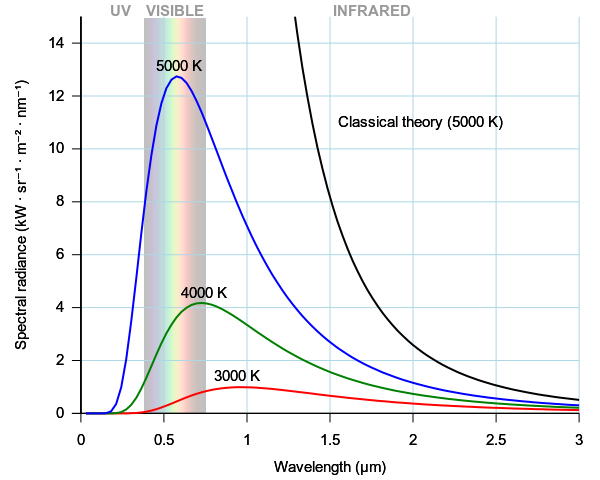
\includegraphics[scale=0.5]{Black_body}
\caption{Blackbody radiation. By Darth Kule - Own work, Public Domain, 
https://commons.wikimedia.org/w/index.php?curid=10555337}
\label{c2f1}
\end{figure}

The plot shows that as temperature
rises the dominant wavelength decreases. It agrees with the observation that
hot bodies successively appear redish to bluish to white as their temperature
increases. Lord Rayleigh and Sir James Jeans first tried to understand the
black body spectrum assuming that radiation is in the form of electromagnetic
waves. Radiation is trapped inside a black body in the form of standing waves.
If we the black body is in the form a cube of length $L$ then radiation of 
wavelength $\lambda$ will stay as a standing wave only if an integral number of
half wavelengths are accommodated in the extent $L$. If $n_x, n_y, n_z$ are the
number of half-wavelengths along the $x, y, z$ axes then
\begin{eqnarray}
n_x &=& \frac{L}{\lambda/2} = \frac{2L}{\lambda} \\
n_y &=& \frac{2L}{\lambda} \\
n_z &=& \frac{2L}{\lambda}
\end{eqnarray}
For a standing wave to form in an arbitrary direction we must have
\begin{equation}\label{c2s1e5}
n^2 = n_x^2 + n_y^2 + n_z^2 = \left(\frac{2L}{\lambda}\right)^2.
\end{equation}
In this equation we no longer require $n_x, n_y, n_z$ to be integers.
The number of waves with wavelengths between $\lambda$ and $\lambda + d\lambda$
is the number of points with positive coordinates $n_x, n_y, n_z$ in the region
between the first octant of the spheres with radii $n$ and $n + dn$. This number
is proportional to the volume of the region,
\[
\frac{1}{8} \times 4\pi n^2dn.
\]
Since there are two polarisations for each mode, the number of standing waves is
\begin{equation}\label{c2s1e6}
G(n)dn = \pi n^2 dn.
\end{equation}
From equation \eqref{c2s1e5} we have
\begin{equation}\label{c2s1e7}
n = \frac{2L}{\lambda} = \frac{2L}{c}\nu
\end{equation}
so that equation \eqref{c2s1e6} becomes
\begin{equation}\label{c2s1e8}
G(\nu)d\nu = \pi \cdot \frac{8L^3}{c^3}\nu^2d\nu.
\end{equation}
If $g(\nu)$ is the number of waves per unit volume, also called the density of
`states', then
\begin{equation}\label{c2s1e9}
g(\nu)d\nu = \frac{8\pi}{c^3}\nu^2 d\nu.
\end{equation}
Finally, in order to get the energy density, Rayleigh and Jeans used the 
classical equipartition theorem that allocates an energy of $kT/2$ to each
degree of freedom. In the case of a single standing wave, there are two degrees
of freedom so that the energy of each mode is
\begin{equation}\label{c2s1e10}
U = kT,
\end{equation}
where $k = 1.38 \time 10^{-23}$ JK${}^{-1}$ is the Boltzmann constant and $T$
is the absolute temperature. The energy density is, therefore,
\begin{equation}\label{c2s1e11}
u(\nu)d\nu = \frac{8\pi kT}{c^3}\nu^2 d\nu.
\end{equation}
One can as well express the energy density $u$ as a function of wavelength and
write
\begin{equation}\label{c2s1e12}
u(\lambda)d\lambda = \frac{8\pi kT}{\lambda^2}d\lambda.
\end{equation}
The experimentally observed energy density spectrum of a black body does not
follow these equations. In particular, when $\lambda \rightarrow 0$, or 
equivalently, $\nu \rightarrow \infty$, $u$ blows up. This feature of the 
function $u$ defined in \eqref{c2s1e10} and \eqref{c2s1e11} is called the
`ultraviolet catastrophe' and it was one of the first evidences to indicate 
that certain experiments cannot be explained by classical physics.

Max Planck's correction to this formula lay in replacing the energy given by
equation \eqref{c2e1e10} with
\begin{equation}\label{c2s1e13}
U = \frac{h\nu}{\exp(\frac{h\nu}{kT}) - 1}
\end{equation}
where $h = 6.626 \times 10^{-34}$ Js is a universal constant, now called the
Planck's constant. The expression for energy density becomes
\begin{equation}\label{c2s1e14}
u(\nu)d\nu = \frac{8\pi h\nu^3}{c^3}\frac{d\nu}{\exp(\frac{h\nu}{kT}) - 1}.
\end{equation}
This is Planck's formula for black body radiation spectrum. 

\subsection{Planck's expression for $U$}
There are many ways to derive Planck's expression in equation \eqref{c2e1e13}
for the energy of radiation. We will follow the one used originally by Planck
\cite{planck1901law}. It assumes
\begin{enumerate}
\item The relation between entropy $S$ and internal energy $U$
\begin{equation}\label{c2s1e15}
\left(\frac{\partial S}{\partial U}\right)_{V, N} = \frac{1}{T}.
\end{equation}
Here $T$ us the (absolute) temperature and $N$ is the number of particles.
\item The relation between entropy and the number of states in which a system
can be. If $\Omega$ is the number of states then
\begin{equation}\label{c2s1e16}
S = k\log\Omega
\end{equation}
where $k$ is another universal Boltzmann constant.
\item Electromagnetic energy is transferred in the units of $h\nu$, where $\nu$
is the frequency of the radiation and $h$ is a universal constant, now named 
after Planck.
\end{enumerate}
Of these assumptions, the first one is a result in thermodynamics, known since 
the 1850s. The second one was proposed by Ludwig Boltzmann in the 1870s when he
laid the foundations of statistical mechanics while the last one was Planck's 
contribution for which he was to receive a Nobel prize in Physics in 1918.

Let the black body cavity have an energy $U_0$ at the frequency $\nu$. If there 
are $N$ modes of radiation, we want to find out the number of ways in which we 
can  distribute the energy $U$ among them. The third assumption listed above 
tells  that the energy $U$ is available as $P=U_0/(h\nu)$ packets, called quanta. 
Therefore, the problem of distribution of energy $U_0$ among the radiation modes
is the same as counting the number of ways in which $P$ quanta can be 
distributed among $N$ modes. This is an easy combinatorial problem whose 
solution is
\begin{equation}\label{c2s1e17}
\Omega = \frac{(P + N - 1)!}{P!(N - 1)!}.
\end{equation}
Usually, the number $N$ is so large that $(N - 1)! \approx N!$ so that we can
as well write \eqref{c2s1e17} as
\begin{equation}\label{c2e1e18}
\Omega = \frac{(P + N)!}{P!N!}.
\end{equation}
so that
\[
\log\Omega = \log[(P + N)!] - \log P! - \log N!.
\]
When $n$ is large, we can approximate $\log n! \approx n\log n$ (this is called
Stirling's approximation. It is quite accurate even for $n = 10$) to get
\[
\log\Omega = (P + N)\log(P + N) - P\log P - N\log N
\]
so that the entropy of the electromagnetic radiation is
\begin{eqnarray*}
S &=& k\log\Omega \\
  &=& kN\left\{\left(1 + \frac{P}{N}\right)\log(P + N) - \frac{P}{N}
      \log P - \log N\right\} \\
 &=& kN\left\{\left(1 + \frac{P}{N}\right)\log(P+N) - \frac{P}{N}
     \left(\log\frac{P}{N} + \log N\right) - \log N\right\} \\
 &=& kN\left\{\left(1 + \frac{P}{N}\right)\left(\log(P+N)-\log N\right)
     - \frac{P}{N}\log\frac{P}{N}\right\} \\
 &=& kN\left\{\left(1 + \frac{P}{N}\right)\log\left(1+\frac{P}{N}\right)
     - \frac{P}{N}\log\frac{P}{N}\right\}
\end{eqnarray*}
Since $P$ was defined as $U_0/(h\nu)$, we can write
\[
\frac{U_0}{Nh\nu} = \frac{U}{h\nu}
\]
where
\begin{equation}\label{c2s1e19}
U = \frac{U_0}{N}
\end{equation}
is the average energy per mode. We now have
\begin{equation}\label{c2s1e20}
S = kN\left\{\left(1 + \frac{U}{h\nu}\right)\log\left(1+\frac{U}{h\nu}\right)
     - \frac{U}{h\nu}\log\frac{U}{h\nu}\right\}.
\end{equation}     
From equations \eqref{c2s1e15} and \eqref{c2s1e19} one can readily show that
\begin{equation}\label{c2s1e21}
\frac{1}{T} = \frac{k}{h\nu}\left(1 + \frac{h\nu}{U}\right).
\end{equation}
This equation can be rearranged to get
\begin{equation}\label{c2s1e22}
U = \frac{h\nu}{\exp\left(\frac{h\nu}{kT}\right) - 1}
\end{equation}
which is identical with \eqref{c2s1e13}.

\subsection{Additional notes on Planck's derivation}
Planck deduced the relation $E = h\nu$ first on the basis of thermodynamic
arguments (section 2 of \cite{planck1901law}). Later on (sixth lecture in 
\cite{planck2012eight}) he gave an explanation using the mathematical 
properties of electromagnetic radiation. Chang \cite{chang2017physical} gives 
an account of Planck's theory in modern terms.

Entropy is usually introduced as a quantity measuring the disorder in a system.
The molecules of a vapour have more freedom of movement than the molecules of a
liquid. As a result we say the vapour has more entropy than a liquid. What could
entropy mean in the case of radiation? Radiation is characterised by frequency 
(or wavelength), phase and amplitude. The entropy of radiation consists in 
random fluctuations of phase and amplitude.

Although Planck introduced the idea of a quantum of energy he did not consider it
as seriously as others like Einstein, Ehrenfest and Lorentz (preface of 
\cite{planck2012eight}). In the remaining sections we will see how the idea 
turned out to have a profound and far-reaching impact on physics.

\subsection{Problem set 1}
\begin{enumerate}
\item Physics is an experimental science. We should supplement the theoretical
development of black body radiation spectrum of \eqref{c2s1e14} with an 
understanding of how it is measured. Refer to 
\url{https://physicsopenlab.org/2015/12/04/black-body-emission/} for one way to
measure the spectrum.
\item When the voltage drops an incandescent bulb gives a reddish glow. When the
voltage reaches its normal level the bulb glows bright. Can you explain the 
change in appearance based on your understanding of \eqref{c2s1e14}?
\item It is safer to use a touchless thermometer when a large number of people
have to be examined. Can you design a touchless thermometer using 
\eqref{c2s1e14}?
\item Consider the function
\begin{equation}\label{c2e1e23}
B(\nu, T) = \frac{2h\nu^3}{c^2}\frac{1}{\exp\left(\frac{h\nu}{kT}\right) - 1}.
\end{equation}
Show that it reaches an extremum at a frequency $\nu_0$ such that
\begin{equation}\label{c2e1e24}
3 + \left(\frac{h\nu_0}{kT} - 3\right)\exp\left(\frac{h\nu_0}{kT}\right) = 0.
\end{equation}
If you measure the radiation spectrum of a body using the procedure outlined
in the first problem and read the frequency $\nu_0$ at which the spectral energy 
density peaks then you can use equation \eqref{c2e1e24} to determine the 
temperature.
\item If 
\begin{equation}\label{c2e1e25}
x = \frac{h\nu_0}{kT}
\end{equation}
then equation \eqref{c2e1e24} can be written as $3 + (x - 3)e^x = 0$. You can
solve this equation using Newton's method to get $x \approx 2.821440$. Thus,
the relation between temperature of the black body and its peak frequency is
\begin{equation}\label{c2s1e26}
\frac{h\nu_0}{kT} \approx 2.821440.
\end{equation}
Using equation \eqref{c2s1e26} find the peak frequency when you measure the
radiation spectrum of
\begin{enumerate}
\item Sun whose surface temperature is approximately $6000$ K?
\item human body with temperature of $310$K? (Do you now see the usefulness
of infrared cameras?)
\end{enumerate}
On the other hand the peak frequency of the outer space is around $160$ GHz.
What is the space's temperature? (The ambient radiation in the outer space 
is called the cosmic microwave background. Can you relate it to the relativistic
Doppler effect you studied in the previous chapter?)
\end{enumerate}